\documentclass[]{beamer}
\mode<presentation>
{
  \usetheme{Warsaw}
  \definecolor{mcgarnet}{rgb}{0.38, 0, 0.08}
  \definecolor{mcgray}{rgb}{0.6, 0.6, 0.6}
  \setbeamercolor{structure}{fg=mcgarnet,bg=mcgray}
  %\setbeamercovered{transparent}
}


\usepackage[english]{babel}
\usepackage[latin1]{inputenc}
\usepackage{times}
\usepackage[T1]{fontenc}
\usepackage{tikz}
\usepackage{graphicx}
\usepackage{syntax}

\newcommand{\imagesource}[1]{{\centering\hfill\break\hbox{\scriptsize Image Source:\thinspace{\small\itshape #1}}\par}}

\title{07 - Lexical Analysis}


\author{Dr. Robert Lowe\\}

\institute[Maryville College] % (optional, but mostly needed)
{
  Division of Mathematics and Computer Science\\
  Maryville College
}

\date[]{}
\subject{}

\pgfdeclareimage[height=0.5cm]{university-logo}{images/Maryville-College}
\logo{\pgfuseimage{university-logo}}



\AtBeginSection[]
{
  \begin{frame}<beamer>{Outline}
    \tableofcontents[currentsection]
  \end{frame}
}


\begin{document}

\begin{frame}
  \titlepage
\end{frame}

\begin{frame}{Outline}
  \tableofcontents
\end{frame}


% Structuring a talk is a difficult task and the following structure
% may not be suitable. Here are some rules that apply for this
% solution: 

% - Exactly two or three sections (other than the summary).
% - At *most* three subsections per section.
% - Talk about 30s to 2min per frame. So there should be between about
%   15 and 30 frames, all told.

% - A conference audience is likely to know very little of what you
%   are going to talk about. So *simplify*!
% - In a 20min talk, getting the main ideas across is hard
%   enough. Leave out details, even if it means being less precise than
%   you think necessary.
% - If you omit details that are vital to the proof/implementation,
%   just say so once. Everybody will be happy with that.

\section{Lexical Analysis}

\begin{frame}{Lexical Analysis Tasks}
    \begin{itemize}[<+->]
        \item The lexical analyzer, or \textbf{lexer}, processes the
            micro-syntax of a language.
        \item The lexer converts sequences of terminals into
            \textbf{lexemes}.
        \item A lexeme is the basic building block of a language.
        \item The lexer has two basic layers/tasks:
        \begin{enumerate}
            \item Scanner
            \item Screener
        \end{enumerate}
    \end{itemize}
\end{frame}

\begin{frame}{Analyzing the Micro-Syntax}
    \begin{itemize}[<+->]
        \item The micro-syntax of a language is the portion of the 
            language which is expressible as a regular grammar.
        \item Recall that regular grammars consist of these productions:
            \newline$A \rightarrow a$ and $A \rightarrow aB$
        \item These productions are the \textbf{lexemes} of
            a language.
        \item Example lexemes include:
            \begin{itemize}
                \item Literals
                \item Identifiers
                \item Keywords
            \end{itemize}
        \item It is possible to use recursive descent for this, but
            this would be overkill for a lexer!
    \end{itemize}
\end{frame}

\begin{frame}{Scanning}
    \begin{itemize}[<+->]
        \item In the scanning layer, the lexer consumes sequences of
            characters and transforms them into the productions of the
            micro-syntax.
        \item Scanning can be implemented as recursive descent, but
            this is not necessary.
        \item Scanning is typically implemented as a simple state
            machine. 
        \item This is also known as ``regular expression parsing'',
            because the language processed by the lexer is a regular
            grammar.
    \end{itemize}
\end{frame}

\begin{frame}{Screening}
    \begin{itemize}[<+->]
        \item Screening is the layer which excludes improper
            characters or sequences of characters.
        \item Usually, screening is done as an exclusionary sort of
            process.
        \item Sometimes screened characters are skipped (for example,
            unneeded whitespace or comments).
        \item If something does not match the rules of the lexer's
            language, it is flagged as an invalid sequence.
    \end{itemize}
\end{frame}

\begin{frame}{The Lexer Interface}
    \begin{itemize}[<+->]
        \item A global variable \texttt{symbol}
        \item \textbf{procedure} \texttt{next\_symbol}
        \begin{itemize}
            \item This is where most of the lexer exists.
            \item Includes the state machine that consumes the input
                stream.
            \item Rather than producing single characters, this 
                procedure will process as many characters as needed
                for the regular productions of the language.
        \end{itemize}
        \item The remaining two procedures provide convenience for
            matching symbols.
            \begin{itemize}
                \item \textbf{procedure} \texttt{mustbe(s)}
                \item \textbf{procedure} \texttt{have(s)}
            \end{itemize}
    \end{itemize}
\end{frame}

\section{Regular Expressions}
\begin{frame}[fragile]{Simple Regular Expression Syntax}
    \begin{itemize}[<+->]
        \item \textbf{grouping}  \texttt{(...)}
        \item \textbf{boolean or} \texttt{a | b}
        \item \textbf{wildcard} \texttt{.}
        \item \textbf{quantifiers} Quantifiers follow a symbol or a
            group and specify how many occurrences match.
            \begin{itemize}
                \item \texttt{*}: zero or more
                \item \texttt{+}: one or more
                \item \texttt{?}: exactly zero or one
            \end{itemize}
        \item \textbf{escaping literals} The special characters in regular
            expressions can all be escaped in the usual way. 
            \newline \verb!\(, \), \|, \., \*, \*, \*, \?, \\!
    \end{itemize}
\end{frame}

\begin{frame}{Regular Expressions and DFA's}
    \begin{itemize}[<+->]
        \item A regular expression is equivalent to a deterministic
            finite automaton (DFA).
        \item A DFA is a graph where states are represented by vertices.
        \item Edges show transitions from each state for a given
            character or set of characters.
        \item For example: \texttt{aa.*b+} becomes the DFA:
            \newline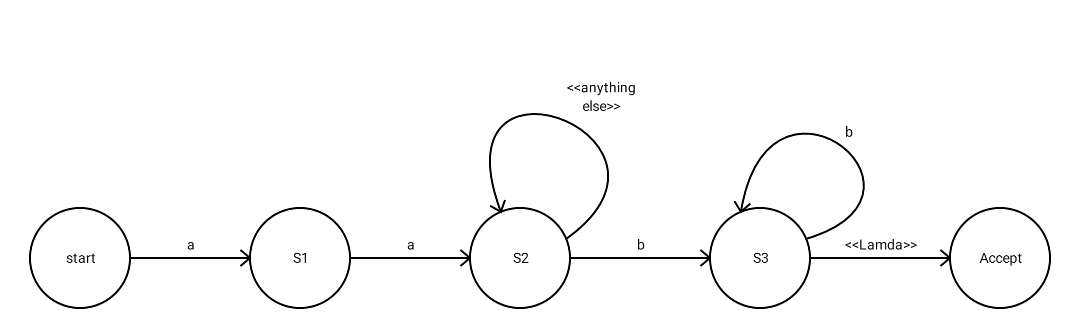
\includegraphics[width=0.9\textwidth]{images/aabdfa} 
    \end{itemize}
\end{frame}

\begin{frame}{Coding a DFA}
    \begin{center}
        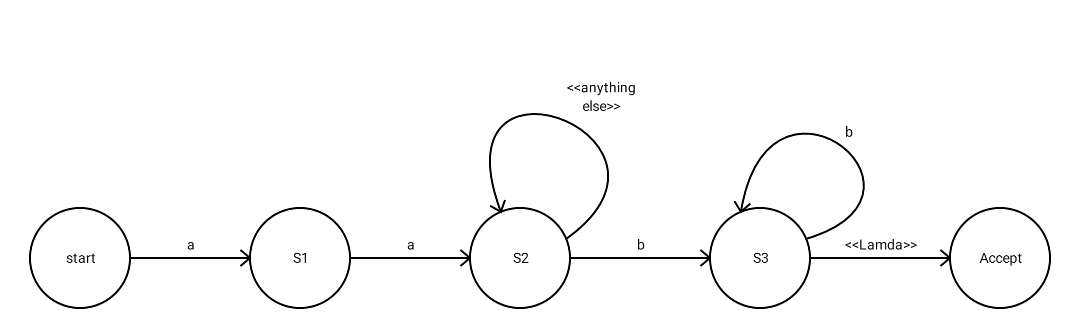
\includegraphics[width=0.9\textwidth]{images/aabdfa} 
    \end{center}
    \begin{itemize}[<+->]
        \item A DFA can be readily converted into code.
        \item First, we need an enumeration for the states.
        \item Then we set the initial state.
        \item Next, we write a loop that will scan the input.
        \item Within the loop, we add \texttt{if} statements to transition the
            state.  Any invalid transition returns an error.
        \item \textbf{Activity}: Let's code the above DFA!
    \end{itemize}
\end{frame}


\section{Tokenization}

\begin{frame}[fragile]{Tokens}
    \begin{itemize}[<+->]
        \item A \textbf{token} is a sequence of characters with
        meaning. (A token is equivalent to a lexeme.)
        \item One approach in C++ would be to represent a token using
            an enumeration:
            \newline\verb!enum Token_Type {INVALID_TOK, OPERATOR_TOK,!
            \newline\verb!                 INTEGER_TOK, LPAREN_TOK,!
            \newline\verb!                 RPAREN_TOK, EOF_TOK};!
        \item We often need to store some additional information about
            a token:
            \newline\verb!struct Token {!
            \newline\verb!    Token_Type type;!
            \newline\verb!    string text;!
            \newline\verb!};!
    \end{itemize}
\end{frame}

\begin{frame}{Identifying Tokens}
    \begin{itemize}[<+->]
        \item Tokens are typically represented by implementing the DFA
            which represents the regular grammar of the lexer.
        \item The basic strategy is this:
            \begin{enumerate}
                \item Set the state to the start state.
                \item Peek at the next character and transition to an
                    appropriate state.
                \item Continue following transitions until the
                    production ends.
                \item Emit the token indicated by the current state.
            \end{enumerate}
    \end{itemize}
\end{frame}

\begin{frame}{Tokenizing a String}
    \begin{itemize}[<+->]
        \item The global \texttt{symbol} variable should be
            a \texttt{Token} structure.
        \item Each call to \texttt{next\_symbol} should perform the 
            DFA on the stream.
        \item \texttt{symbol} is set to the emitted token.
    \end{itemize}
\end{frame}


\section{L++}

\begin{frame}{The Grammar of L++}
\begin{grammar}
    <program> ::= <expression>

    <expression> ::= <term> <expression-tail>
    
    <expression-tail> ::= $\lambda$ | '+' <term> <expression-tail>
    
    <term> ::= <factor> <term-tail>
    
    <term-tail> ::= $\lambda$ | '*' <factor> <term-tail>
    
    <factor> ::= <integer> | '(' <expression> ')'

    <integer> ::= <unit> | <unit><integer>
    
    <unit> ::= '0' | '1' | '2' | '3' | '4' | '5' | '6' | '7' | '8'
    | '9'
\end{grammar}
\end{frame}


\begin{frame}[fragile]{Regular Expressions of L++}
    \begin{itemize}[<+->]
        \item \verb!integer := (0|1|2|3|4|5|6|7|8|9)+!
        \item \verb!operator := +|*!
        \item \verb!lparen := \(!
        \item \verb!rparen := \)!
        \item \verb!invalid := ! anything else.
    \end{itemize}
\end{frame}

\begin{frame}{L++ DFA}
    \begin{center}
        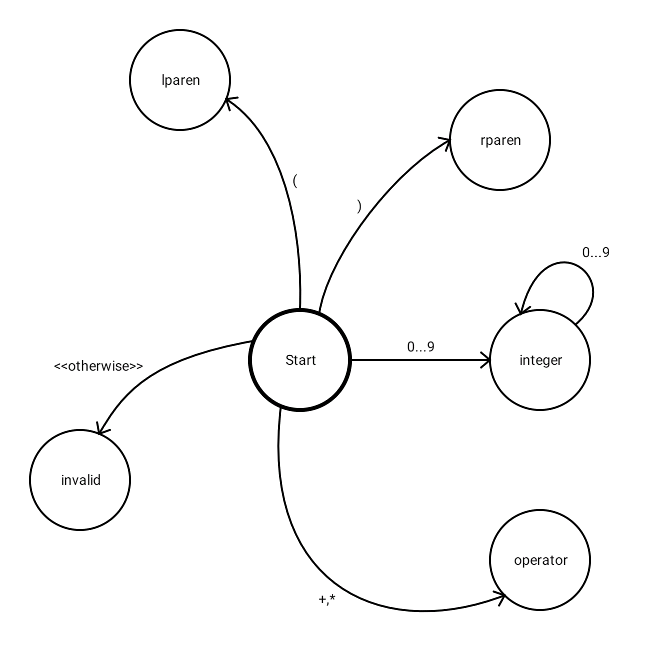
\includegraphics[height=0.95\textheight]{images/lpp}
    \end{center}
\end{frame}

\end{document}


